
%%
%% Template chap2.tex
%%

\chapter{Experiment 2: Learning with Thompson Sampling}
\label{cha:expt2}

Let us now turn our attention to active learning. In this chapter, we investigate the six active
learning heuristics described in section \ref{sec:heuristics}: two uncertainty sampling heuristics
(entropy and margin), two version space reduction heuristics (QBB margin and QBB KL), variance
minimisation, and classifier certainty. We then use Thompson sampling to see if it can
automatically filter out the bad heuristics and select the optimal ones.


\section{Experimental Protocol}
\label{sec:protocol2}

Out of the four classifiers studied in Chapter \ref{cha:expt1}, only logistic regression and RBF
SVMs provide reliable probability estimates. Random forests are able to predict class probabilities
by looking at the distribution of votes. However, we find in practice that they are not stable.
With linear SVMs, the probability functionality has not been implemented in scikit-learn. Thus we
are left with only two choices: logistic regression and RBF SVMs. The hyperparameters of these
classifiers are the same as those in the previous chapter.

For the unlabelled pool, we examine two cases. In one case, the pool is balanced, with an equal
number of objects in each class. This allows us to find out the maximum performance of the
heuristics in the best possible scenario. Of course, in real life, the classes are not evenly
distributed. Thus in the second case, we keep the original class distribution and see if the
performance would deteriorate in any way.

Given two choices of classifiers and two ways to construct the unlabelled pool, we have in total
four variations for each dataset and heuristic. In each run, we do a stratified shuffle split of
the training and test data with 10 trials. For the SDSS data, the training and test sets each
contain 10,000 examples in each split. For the VST ATLAS data, each split uses 70\% of all the
available data (or 24,539 objects) for training and the remaining (10,516 objects) for testing.
So that we can have a meaningful comparison, a random seed is used to make sure that the same
splits are used for all the variations and heuristics.

All heuristics require probability estimates. Thus we need to start with a partially trained
classifier. Initially, 50 random examples are chosen for training. We find that any number smaller
than this would result in a very poor hypothesis with unreliable probability estimates, and if we
pick a number that is too high, the learning curves might be less interesting. A starting sample of
size 50 seems to be a good balance.

Some clarification about the terminology is needed. In this chapter, the training set is used as
the unlabelled pool. In other words, we initially pretend that we do not have any labels for
objects in the training set yet, except for the initial seed of 50 examples. In each round, the
active learner is only allowed to assign a score and label objects in this set. The test set is
hidden away from the active learner and is used to calculate the posterior balanced accuracy at the
end of each round. This can then be used to make the learning curves.

The values of the following parameters are chosen so that the experiments can finish in a reasonable
amount of time:
\begin{itemize}
    \item $E = 300$: In each round, we pick 300 random objects from the pool to be ranked.
    
    \item $n = 300$: We only run each active learning experiment until have 300 labelled
    objects in the training set.
    
    \item $B = 11$: For the two heuristics that require a committee of classifiers, QBB margin and
    QBB KL, we choose a committee of size 11.
    
    \item Finally, the pool variance and pool entropy heuristics require the estimation of the
    variance and the entropy, respectively, of the entire unlabelled pool. Given that this is quite
    an expensive computation, we only select a sample of 300 from the unlabelled pool.
\end{itemize}
In Thompson sampling, we also need to start with some prior knowledge and a likelihood variance:
\begin{itemize}
    \item $\mu_i = 0$: Since initially, we know nothing about the performance of the heuristics, it
    is reasonable to set the prior mean of the mean reward of all heuristics to zero.
    
    \item $\sigma^2_i = \tau^2_i = 0.02$: An arbitrarily small non-zero number is chosen for the prior and
    the likelihood variances. These values should not be zero, since otherwise we would not be able
    to update our beliefs.
\end{itemize}


\section{Results and Discussion}
\label{sec:results2}

We split the discussion of the results into two parts. We first focus on how well active
learning does with the SDSS dataset (Section \ref{sub:learnsdss}). We then examine
the results with the VST ATLAS data (Section \ref{sub:learnvstatlas}), which is much cleaner
but has a rare class of white dwarfs. For each dataset, the discussion is accompanied by
seven pages of visualisations. These are
    \begin{enumerate}
        \item Violin plots of the posterior balanced accuracy distribution after 300 objects 
        have been labelled: These plots give us a quick visual glance of how well the heuristics
        perform relative to each other.
        
        \item Average learning curves of heuristics that perform worse than random sampling.
        
        \item Average learning curves of heuristics that perform better than random sampling: We separate
        out the bad heuristics from the good ones mainly to avoid clutter in the plots.
        
        \item Plots showing the total number of selections of the six heuristics in Thompson sampling:
        These allow us to see how well the Thompson sampling algorithm balances between exploration
        and exploitation.
        
        \item Plots of the selection frequencies of the six heuristics in Thompson sampling.
        
        \item Plots of cumulative rewards of the six heuristics in Thompson sampling.
        
        \item Plots of the mean rewards of the six heuristics in Thompson sampling.
    \end{enumerate}
To make the comparison easier, we have associated each heuristic with the same colour throughout all
the plots. The are also two more sets of visualisations which we put in Appendix \ref{cha:supp}.

\subsection{Learning with the SDSS Dataset}
\label{sub:learnsdss}

Figures \ref{fig:sdss_bl_ind} to \ref{fig:sdss_avg_rewards} show the results of the experiment on
the SDSS dataset. Overall, margin and QBB margin have consistently been the top two heuristics.
They can outperform random sampling by as much as 2\%. QBB margin appears to be no worse the the
simple margin approach. This is expected since the bagging technique has been shown to improve the
stability of the predictions \cite{breiman96}.

The QBB KL heuristic gives a very poor result in logistic regression, while it is comparable with
random sampling in RBF SVMs. The pool variance heuristic is derived from the Taylor series
approximation of multinomial logistic regression and it seems to work reasonably well with the
one-vs-rest strategy. As we would expect, the theory of SVMs are completely different from that of
logistic regression, making the pool variance heuristic unsuitable here. It is interesting to see
that the pool entropy heuristic also performs quite badly with SVMs, while the uncertainty sampling
entropy approach does very well. Finally whether the original data pool is balanced or unbalanced
seems to have a very little effect on the outcome.

For the Thompson sampling, it seems that even under the very simplifying assumption of a normal
prior and a normal likelihood, the algorithm still manages to automatically detect the optimal
heuristic. In most cases, the algorithm discovers the margin heuristic to be optimal after only
around 50 samples. Although Thompson sampling does not perform as well as using the margin heuristic
alone, this is expected since it needs to do some exploration. Still, it gives us the third best
learning curve in all cases, after margin and QBB margin. Finally, there is indeed the problem of
drifting in the mean of the rewards. It would be interesting to find out how much quicker the
algorithm can recognise the optimal heuristic if we were to implement the Dynamic Thompson Sampling
method.


\begin{figure}[p]
	\centering
	\begin{subfigure}{\textwidth}
		\centering
		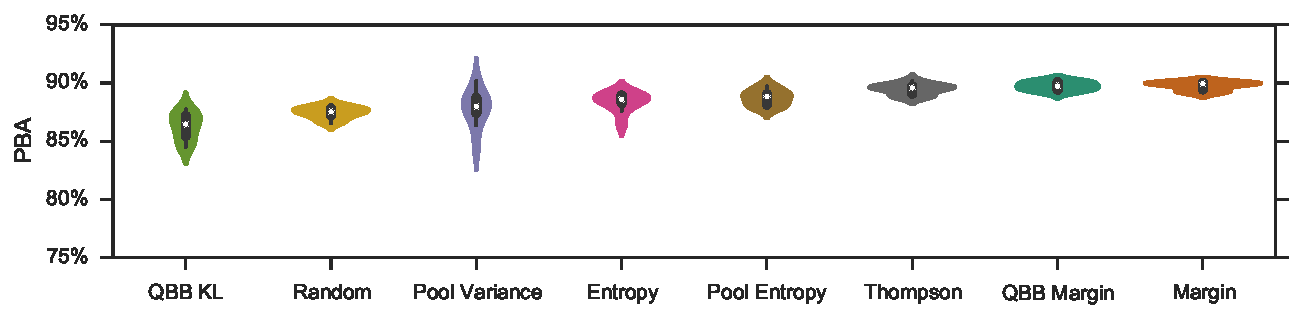
\includegraphics[width=\textwidth]{figures/5_active/sdss_bl_ind_violin}
		\caption{Balanced pool and logistic regression}
		\label{fig:sdss_bl_ind_violin}
	\end{subfigure}
	\begin{subfigure}{\textwidth}
		\centering
		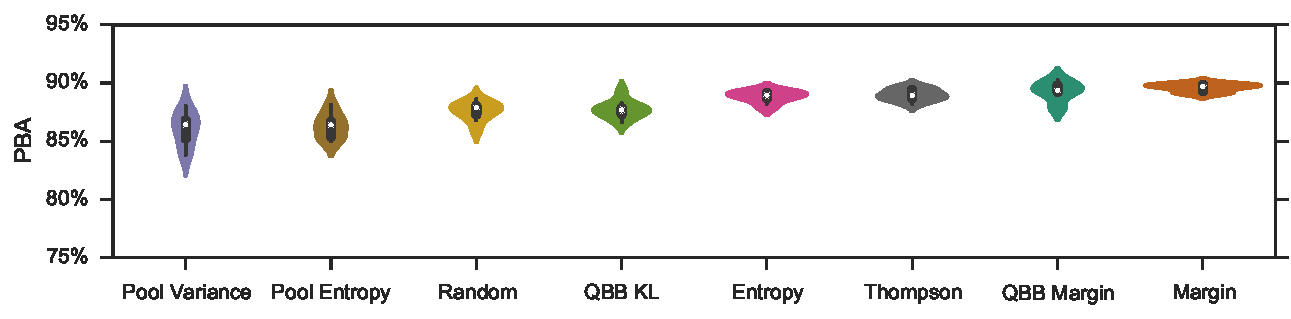
\includegraphics[width=\linewidth]{figures/5_active/sdss_br_ind_violin}
		\caption{Balanced pool and RBF SVM}
		\label{fig:sdss_br_ind_violin}
	\end{subfigure}
	\begin{subfigure}{\textwidth}
		\centering
		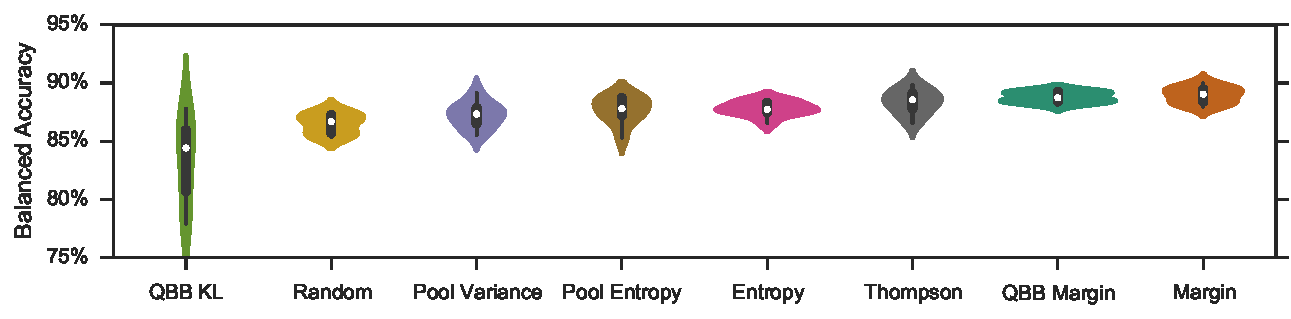
\includegraphics[width=\textwidth]{figures/5_active/sdss_ul_ind_violin}
		\caption{Unbalanced pool and logistic regression}
		\label{fig:sdss_ul_ind_violin}
	\end{subfigure}
	\begin{subfigure}{\textwidth}
		\centering
		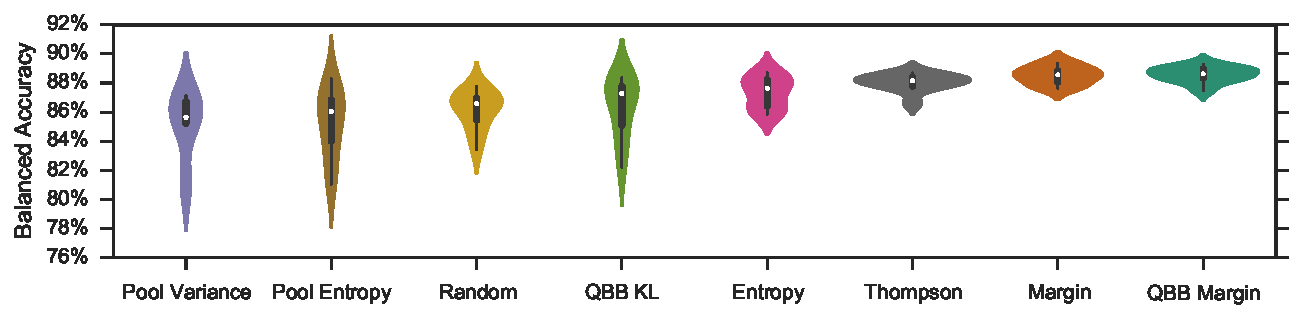
\includegraphics[width=\linewidth]{figures/5_active/sdss_ur_ind_violin}
		\caption{Unbalanced pool and RBF SVM}
		\label{fig:sdss_ur_ind_violin}
	\end{subfigure}
	\caption[Violin plots of balanced accuracy (SDSS)]{Posterior distributions of the balanced
        accuracy when the SDSS training set size reaches 300: Overall, with the exception of QBB KL
        and pool variance, all the other heuristics manage to outperform random sampling. Both margin and
        QBB margin are consistently in the top two, with Thompson sampling always at third place. This is
        expected since there is always some exploration in Thompson sampling. Although the pool variance
        heuristic on average outperforms random sampling slightly, it has a large dispersion and thus
        unreliable.} \label{fig:sdss_bl_ind}
\end{figure}


\begin{figure}[p]
	\centering
	\begin{subfigure}{.5\textwidth}
		\centering
		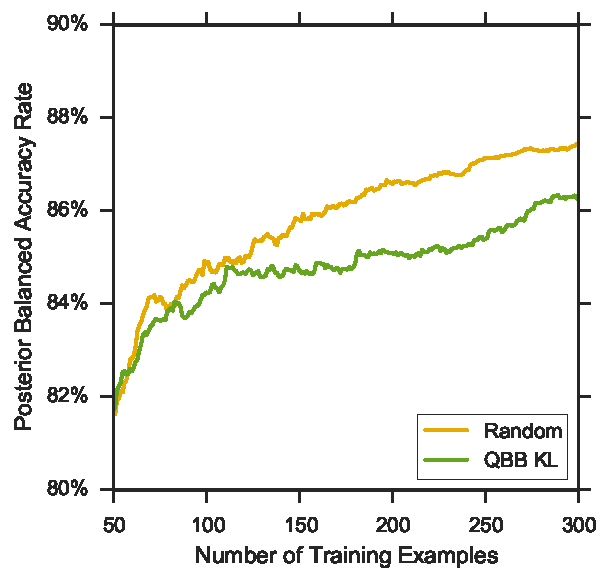
\includegraphics[width=\textwidth]{figures/5_active/sdss_bl_ind_lower}
		\caption{Balanced pool and logistic regression}
		\label{fig:sdss_bl_ind_lower}
	\end{subfigure}%
	\begin{subfigure}{.5\textwidth}
		\centering
		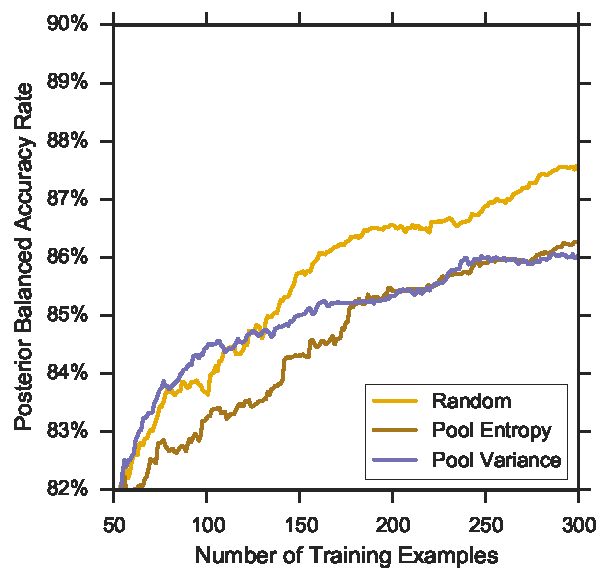
\includegraphics[width=\linewidth]{figures/5_active/sdss_br_ind_lower}
		\caption{Balanced pool and RBF SVM}
		\label{fig:sdss_br_ind_lower}
	\end{subfigure}
	\begin{subfigure}{.5\textwidth}
		\centering
		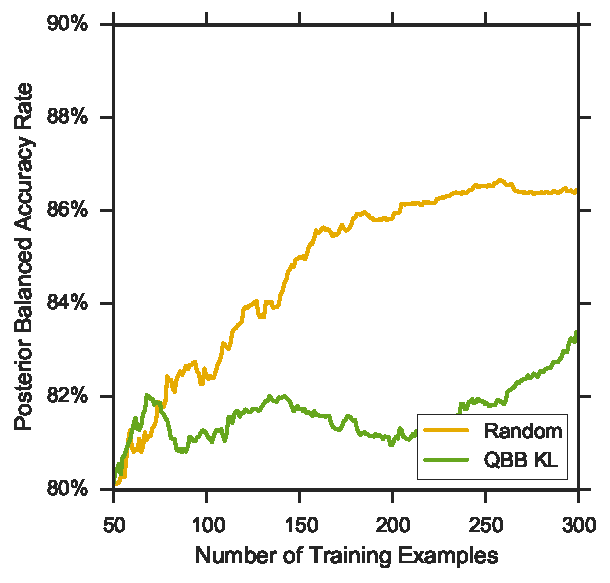
\includegraphics[width=\textwidth]{figures/5_active/sdss_ul_ind_lower}
		\caption{Unbalanced pool and logistic regression}
		\label{fig:sdss_ul_ind_lower}
	\end{subfigure}%
	\begin{subfigure}{.5\textwidth}
		\centering
		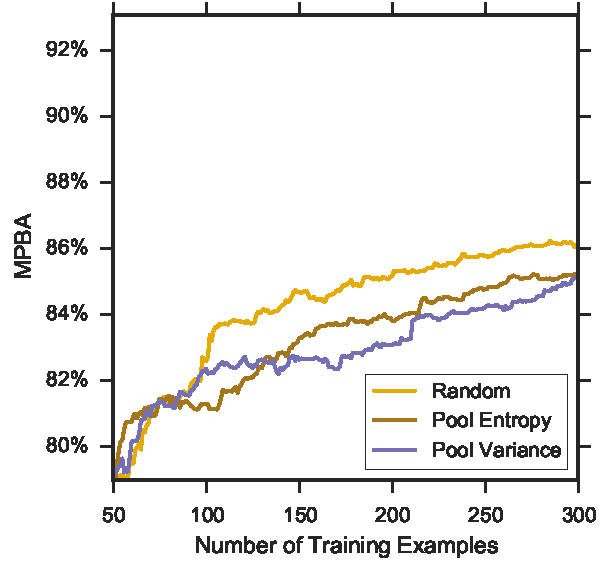
\includegraphics[width=\linewidth]{figures/5_active/sdss_ur_ind_lower}
		\caption{Unbalanced pool and RBF SVM}
		\label{fig:sdss_ur_ind_lower}
	\end{subfigure}
	\caption[Learning curves of heuristics worse than random (SDSS)]{ Learning curves (average of 10
        trials) of heuristics that perform worse than random sampling in the SDSS dataset: We can clearly
        see that with logistic regression, QBB KL performs much worse than random sampling. For RBF SVM,
        the bad heuristics are pool variance and pool entropy. The underperformance of the pool variance
        heuristic is expected since the theory does not quite apply to SVMs. The dashed line is the maximum
        accuracy achievable by the classifier (i.e. the maximum value of the learning curve in Chapter
        \ref{cha:expt1})} \label{fig:sdss_ind_lower}
\end{figure}


\begin{figure}[p]
	\centering
	\begin{subfigure}{.5\textwidth}
		\centering
		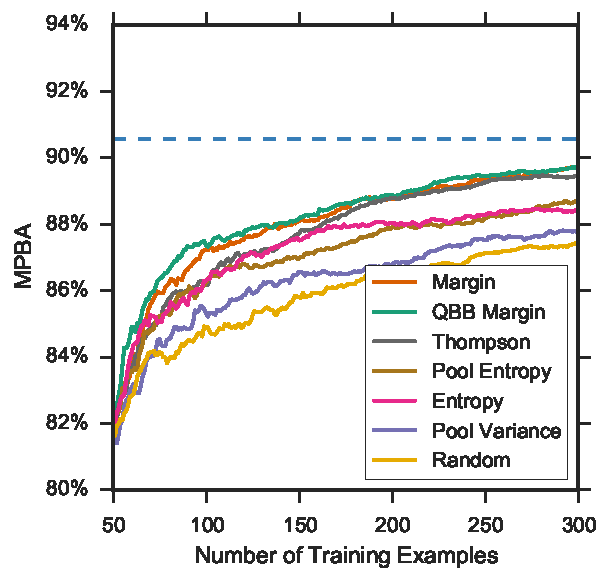
\includegraphics[width=\textwidth]{figures/5_active/sdss_bl_ind_upper}
		\caption{Balanced pool and logistic regression}
		\label{fig:sdss_bl_ind_upper}
	\end{subfigure}%
	\begin{subfigure}{.5\textwidth}
		\centering
		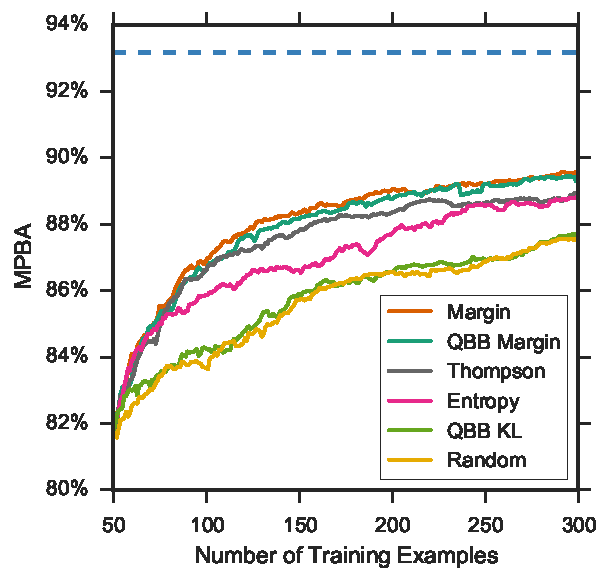
\includegraphics[width=\linewidth]{figures/5_active/sdss_br_ind_upper}
		\caption{Balanced pool and RBF SVM}
		\label{fig:sdss_br_ind_upper}
	\end{subfigure}
	\begin{subfigure}{.5\textwidth}
		\centering
		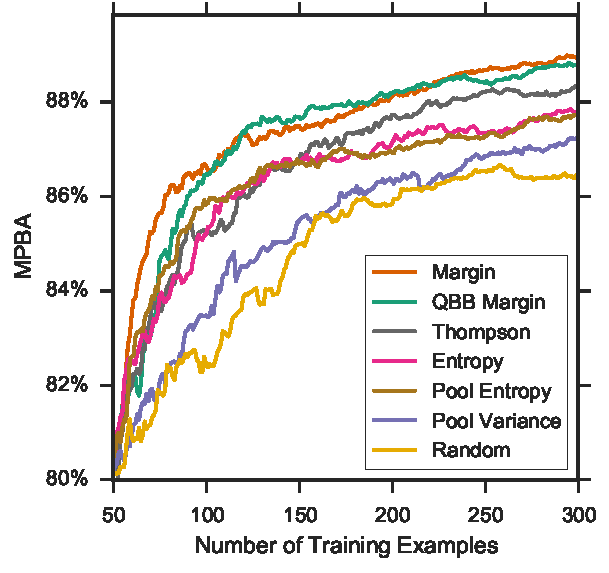
\includegraphics[width=\textwidth]{figures/5_active/sdss_ul_ind_upper}
		\caption{Unbalanced pool and logistic regression}
		\label{fig:sdss_ul_ind_upper}
	\end{subfigure}%
	\begin{subfigure}{.5\textwidth}
		\centering
		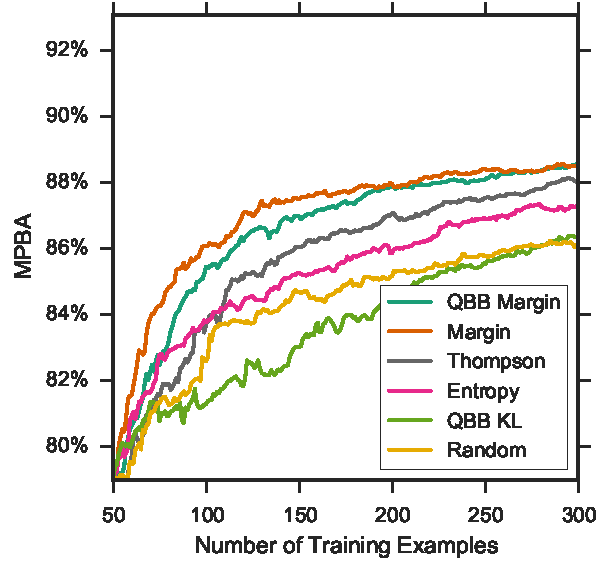
\includegraphics[width=\linewidth]{figures/5_active/sdss_ur_ind_upper}
		\caption{Unbalanced pool and RBF SVM}
		\label{fig:sdss_ur_ind_upper}
	\end{subfigure}
	\caption[Learning curves of heuristics better than random (SDSS)]{Learning curves (average of 10
        trials) of heuristics that outperform random sampling in the SDSS dataset: Again the dashed line
        represents the maximum accuracy achievable by the classifier. Although the learning curves of RBF
        SVM have a lot more potential to go higher, when the sample size is small, its performance is not
        much different from logistic regression, even with active learning. Another interesting
        observation is that with the unbalanced pool and RBF SVM, the QBB KL heuristic is worse than
        random sampling initially but has managed to surpass it just before 300 samples. It would be
        interesting to see their relative performance as we go beyond 300.} \label{fig:sdss_ind_upper}
\end{figure}


\begin{figure}[p]
    \centering
    \begin{subfigure}{.5\textwidth}
        \centering
        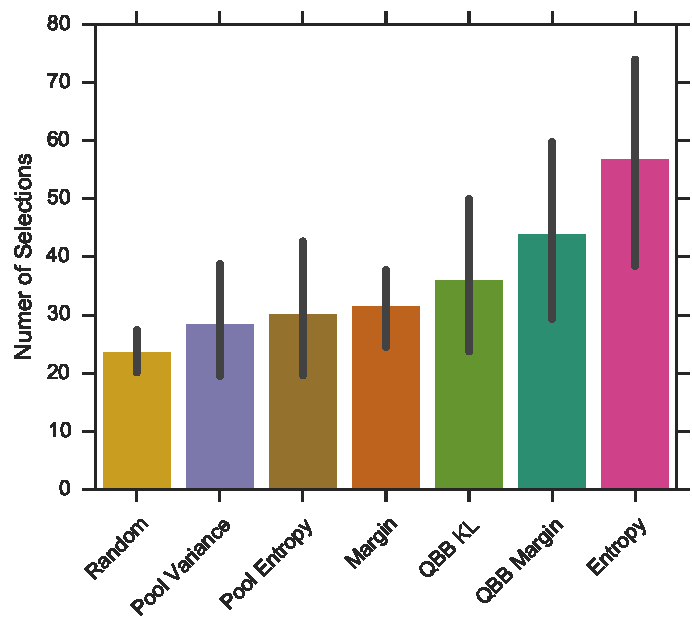
\includegraphics[width=\textwidth]{figures/5_thompson/vstatlas_bl_no_selections}
        \caption{Balanced pool and logistic regression}
        \label{fig:sdss_bl_no_selections}
    \end{subfigure}%
    \begin{subfigure}{.5\textwidth}
        \centering
        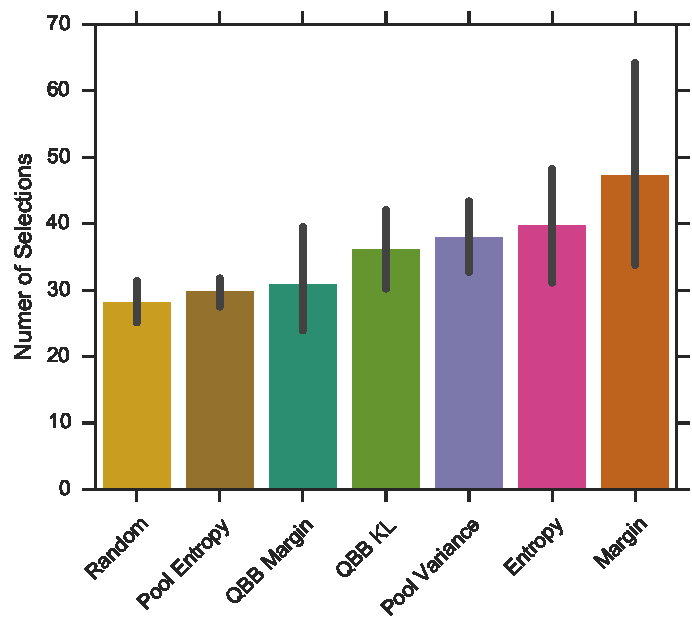
\includegraphics[width=\linewidth]{figures/5_thompson/sdss_br_no_selections}
        \caption{Balanced pool and RBF SVM}
        \label{fig:sdss_br_no_selections}
    \end{subfigure}
    \begin{subfigure}{.5\textwidth}
        \centering
        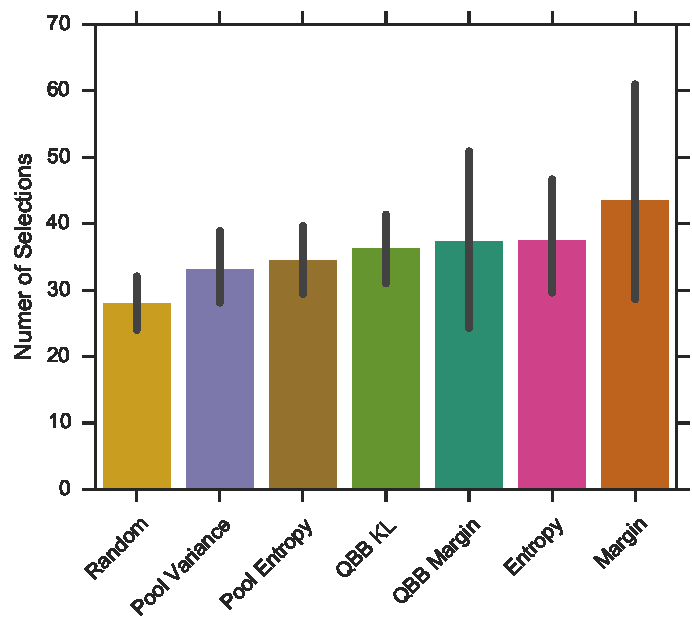
\includegraphics[width=\textwidth]{figures/5_thompson/sdss_ul_no_selections}
        \caption{Unbalanced pool and logistic regression}
        \label{fig:sdss_ul_no_selections}
    \end{subfigure}%
    \begin{subfigure}{.5\textwidth}
        \centering
        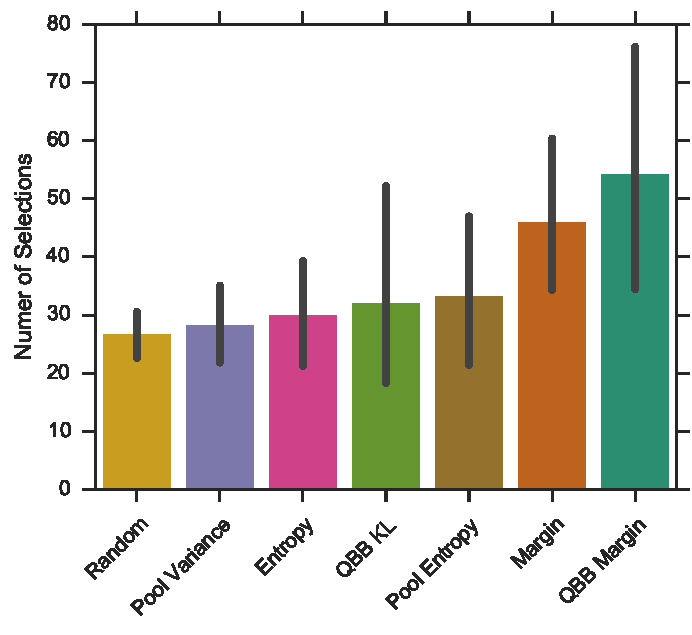
\includegraphics[width=\linewidth]{figures/5_thompson/sdss_ur_no_selections}
        \caption{Unbalanced pool and RBF SVM}
        \label{fig:sdss_ur_no_selections}
    \end{subfigure}
    \caption[Total number of heuristic selections (SDSS)]{Total number of selections (average of 10
        trials) of the six heuristics in Thompson sampling with the SDSS dataset: It seems that
        Thompson sampling has managed to select the better heuristics slightly more often. There also a
        reasonable amount of exploration.} \label{fig:sdss_no_selections}
\end{figure}


\begin{figure}[p]
	\centering
	\begin{subfigure}{.5\textwidth}
		\centering
		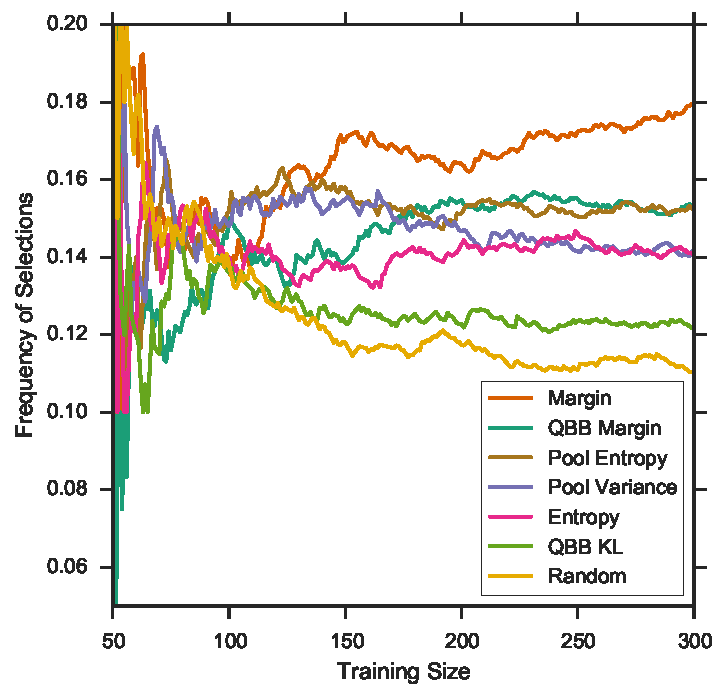
\includegraphics[width=\textwidth]{figures/5_thompson/sdss_bl_frequencies}
		\caption{Balanced pool and logistic regression}
		\label{fig:sdss_bl_frequencies}
	\end{subfigure}%
	\begin{subfigure}{.5\textwidth}
		\centering
		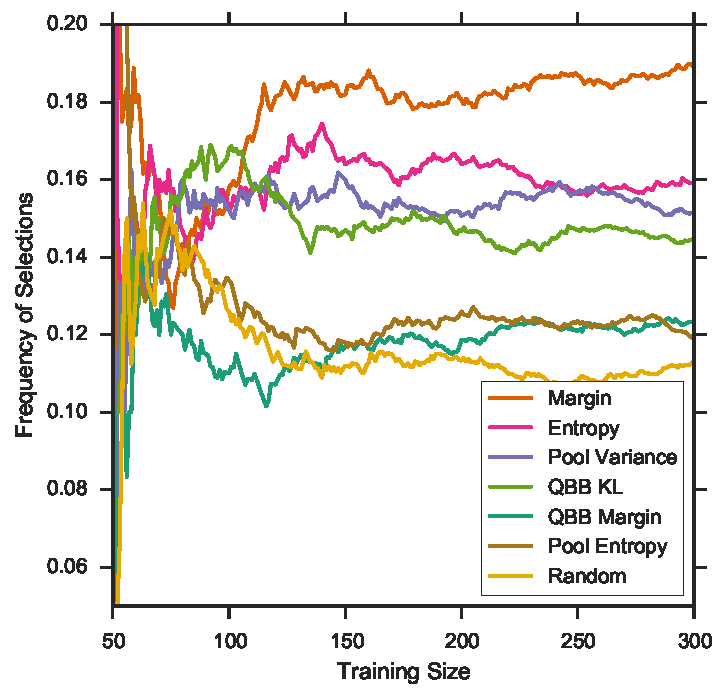
\includegraphics[width=\linewidth]{figures/5_thompson/sdss_br_frequencies}
		\caption{Balanced pool and RBF SVM}
		\label{fig:sdss_br_frequencies}
	\end{subfigure}
	\begin{subfigure}{.5\textwidth}
		\centering
		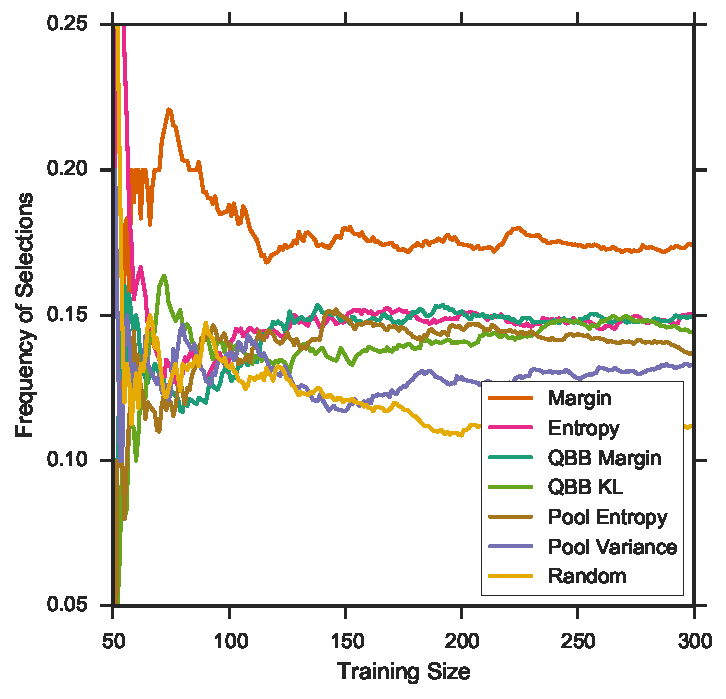
\includegraphics[width=\textwidth]{figures/5_thompson/sdss_ul_frequencies}
		\caption{Unbalanced pool and logistic regression}
		\label{fig:sdss_ul_frequencies}
	\end{subfigure}%
	\begin{subfigure}{.5\textwidth}
		\centering
		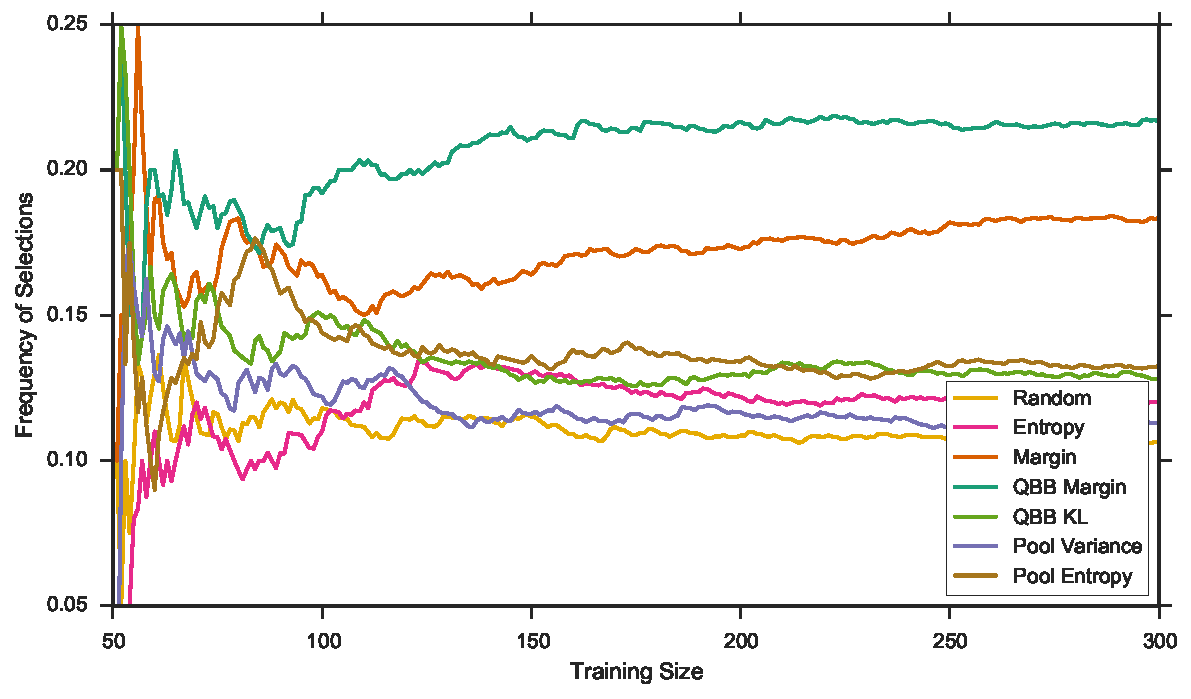
\includegraphics[width=\linewidth]{figures/5_thompson/sdss_ur_frequencies}
		\caption{Unbalanced pool and RBF SVM}
		\label{fig:sdss_ur_frequencies}
	\end{subfigure}
	\caption[Heuristic selection frequency (SDSS)]{ Heuristic selection frequency (average of 10
        trials) in Thompson sampling with the SDSS dataset: Here we get a better look of how the selection
        frequency changes with the sample size. After only around 20 round, the algorithm has managed to
        identify to optimal heuristics like margin.} \label{fig:sdss_frequencies}
\end{figure}


\begin{figure}[p]
	\centering
	\begin{subfigure}{.5\textwidth}
		\centering
		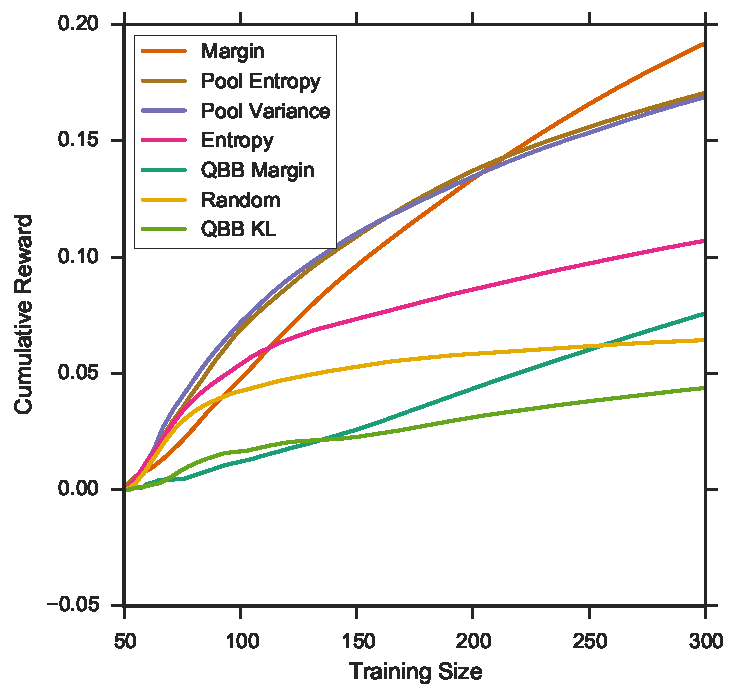
\includegraphics[width=\textwidth]{figures/5_thompson/sdss_bl_sum_rewards}
		\caption{Balanced pool and logistic regression}
		\label{fig:sdss_bl_sum_rewards}
	\end{subfigure}%
	\begin{subfigure}{.5\textwidth}
		\centering
		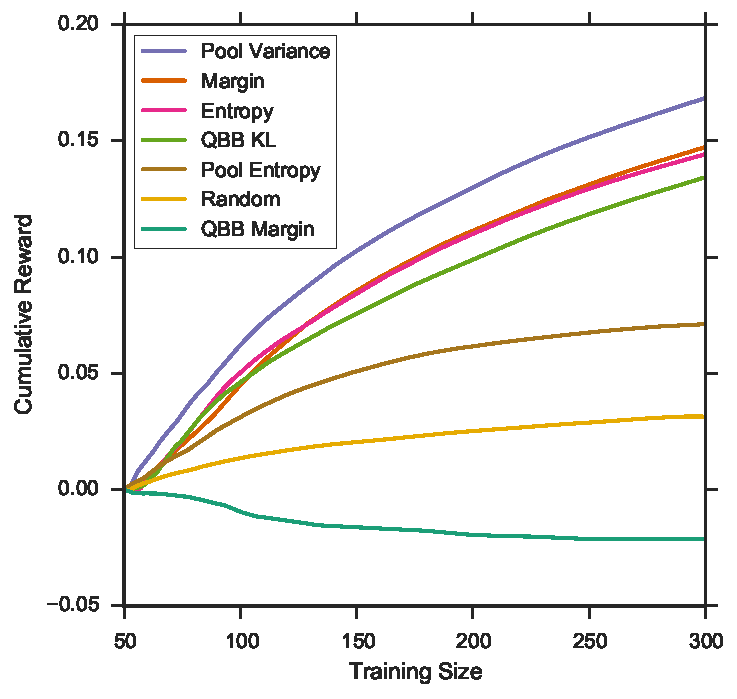
\includegraphics[width=\linewidth]{figures/5_thompson/sdss_br_sum_rewards}
		\caption{Balanced pool and RBF SVM}
		\label{fig:sdss_br_sum_rewards}
	\end{subfigure}
	\begin{subfigure}{.5\textwidth}
		\centering
		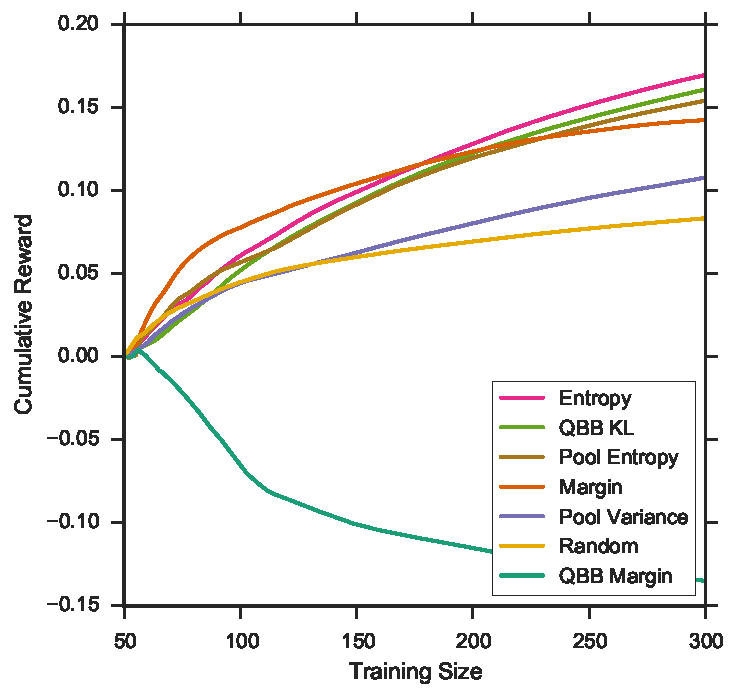
\includegraphics[width=\textwidth]{figures/5_thompson/sdss_ul_sum_rewards}
		\caption{Unbalanced pool and logistic regression}
		\label{fig:sdss_ul_sum_rewards}
	\end{subfigure}%
	\begin{subfigure}{.5\textwidth}
		\centering
		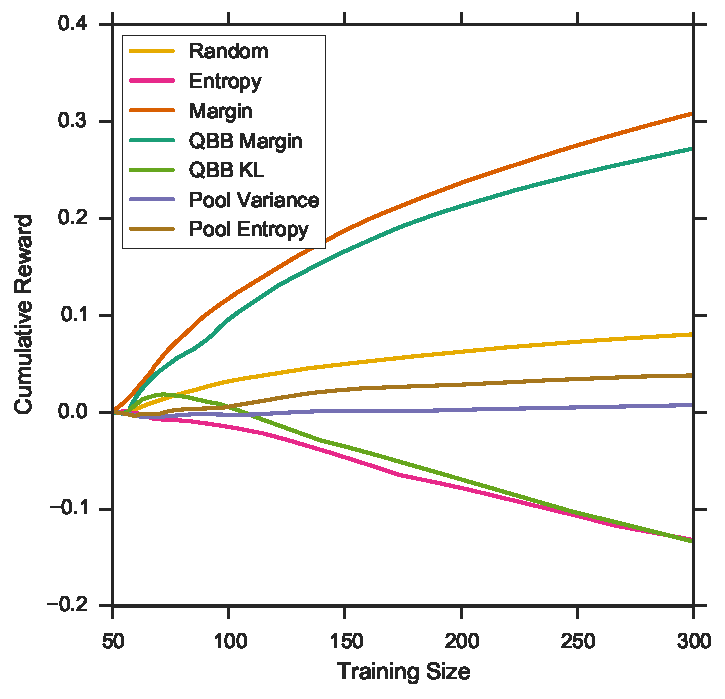
\includegraphics[width=\linewidth]{figures/5_thompson/sdss_ur_sum_rewards}
		\caption{Unbalanced pool and RBF SVM}
		\label{fig:sdss_ur_sum_rewards}
	\end{subfigure}
	\caption[Cumulative reward of heuristics (SDSS)]{
		Cumulative reward (average of 10 trials) in Thompson sampling with the SDSS dataset: One anomaly is with the unbalanced pool and logistic regression, where the average cumulative reward of QBB margin is very low. However, it is supposed to be the second best heuristic. This could simply be due to the averaging process, in which the result is skewed due to an unlucky round. In such rounds, QBB margin might give an unusually low reward (resulting in a false belief).}
	\label{fig:sdss_sum_rewards}
\end{figure}


\begin{figure}[p]
	\centering
	\begin{subfigure}{.5\textwidth}
		\centering
		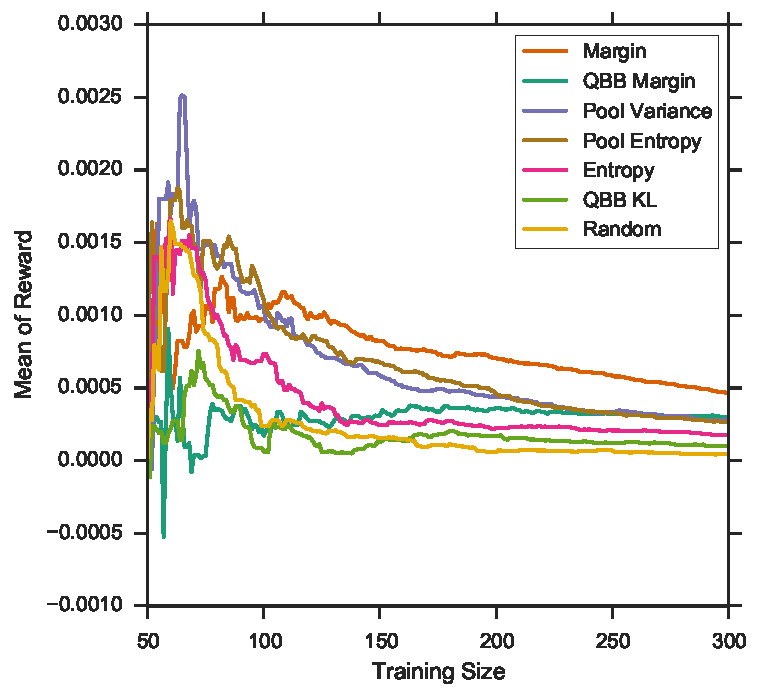
\includegraphics[width=\textwidth]{figures/5_thompson/sdss_bl_avg_rewards}
		\caption{Balanced pool and logistic regression}
		\label{fig:sdss_bl_avg_rewards}
	\end{subfigure}%
	\begin{subfigure}{.5\textwidth}
		\centering
		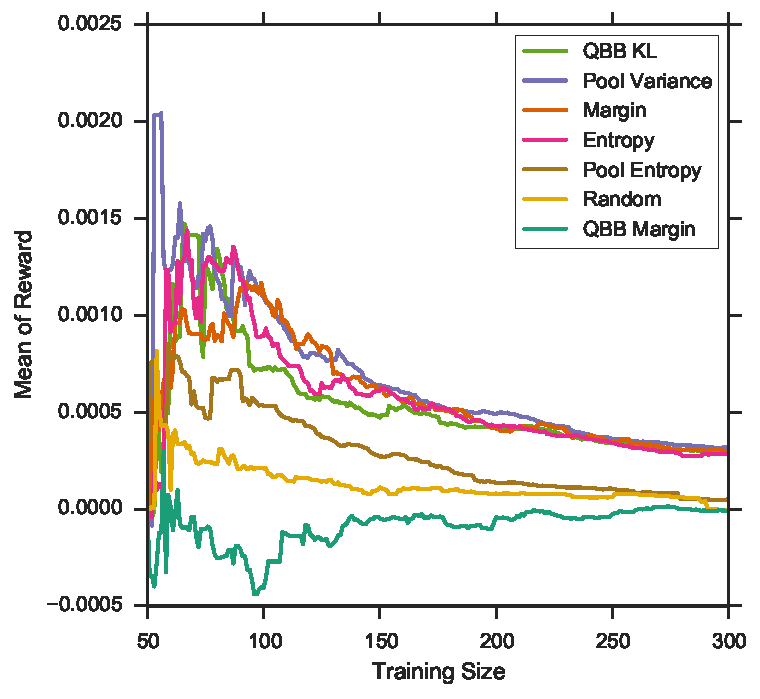
\includegraphics[width=\linewidth]{figures/5_thompson/sdss_br_avg_rewards}
		\caption{Balanced pool and RBF SVM}
		\label{fig:sdss_br_avg_rewards}
	\end{subfigure}
	\begin{subfigure}{.5\textwidth}
		\centering
		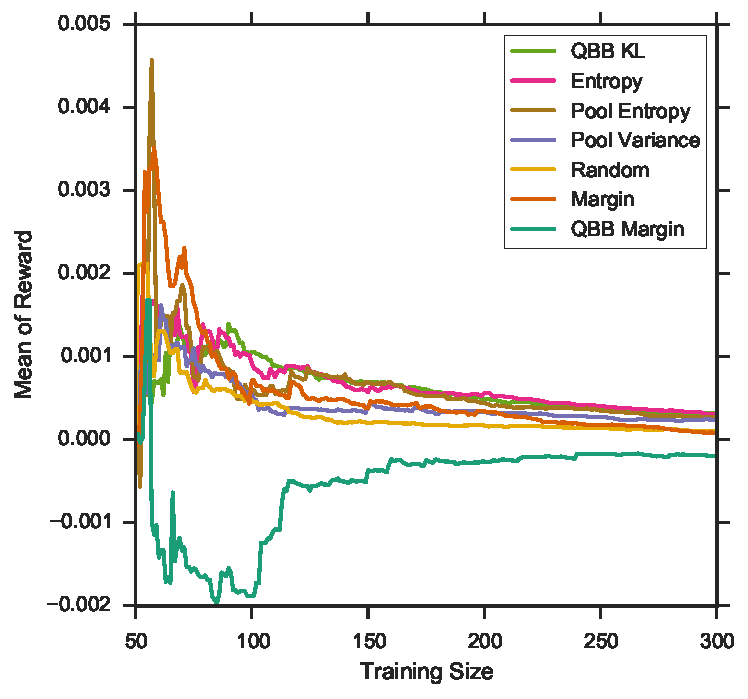
\includegraphics[width=\textwidth]{figures/5_thompson/sdss_ul_avg_rewards}
		\caption{Unbalanced pool and logistic regression}
		\label{fig:sdss_ul_avg_rewards}
	\end{subfigure}%
	\begin{subfigure}{.5\textwidth}
		\centering
		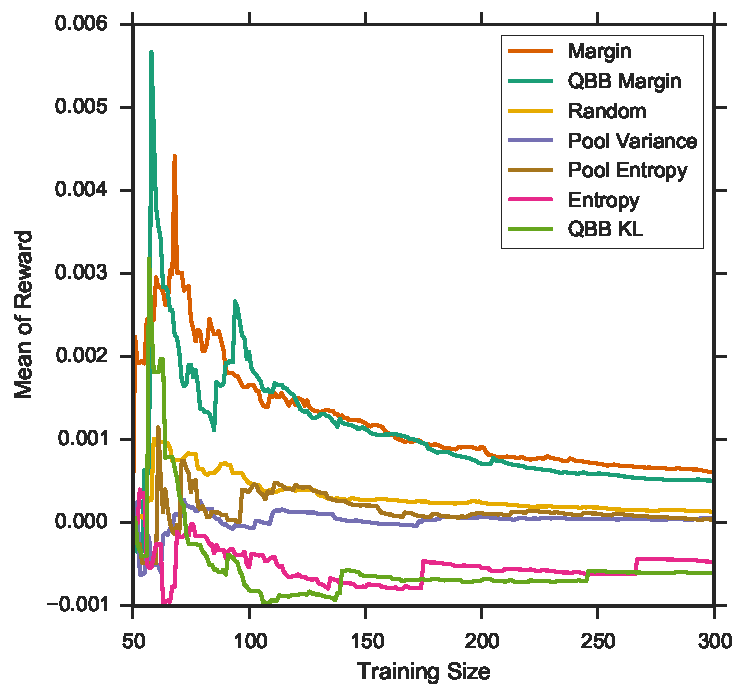
\includegraphics[width=\linewidth]{figures/5_thompson/sdss_ur_avg_rewards}
		\caption{Unbalanced pool and RBF SVM}
		\label{fig:sdss_ur_avg_rewards}
	\end{subfigure}
	\caption[Mean reward of heuristics (SDSS)]{
		Mean reward (average of 10 trials) in Thompson sampling with the SDSS dataset: As expected, the rewards do become smaller over time and drift toward zero.}
	\label{fig:sdss_avg_rewards}
\end{figure}


% % % % % % % % % % % % % % % % % % % % % % % % % % % % % % % % % % % % % % % % % % % % % % % % % %
\subsection{Learning with the VST ATLAS Dataset}
\label{sub:learnvstatlas}

Figures \ref{fig:vstatlas_bl_ind} to \ref{fig:vstatlas_avg_rewards} show the results of the
experiment on the VST ATLAS dataset. The VST ATLAS is a much cleaner dataset, and the active
learning seems to work much better here. Margin, QBB margin, and entropy all perform much better
than random sampling. At times, especially when the dataset is unbalanced, the difference in the
performance can be as great as 9\%. This is a great result since in practice, most datasets have
unbalanced classes.

Thompson sampling is still doing well. Even with the unbalanced pool and logistic regression, where
the algorithm underestimates the usefulness of QBB margin, Thompson sampling still manages to
finish third at the end. This is actually a great feature since it means that it is not necessary
for Thompson sampling to rank all the heuristics in the exact same order as the order that we get
when we study the heuristics individually. A small amount of false belief does not seem to hurt its
overall performance.

Finally, depending on the setting, the three worst heuristics are pool variance, pool entropy and
QBB KL. Often these heuristics are even worse than random sampling. In a way, this is actually good
news because they are also the three most computationally expensive heuristics and thus they are
not very practical anyway. In particular, even when we run the pool variance and the pool entropy
heuristics on the Amazon Elastic Compute Cloud using 36 virtual CPU cores, it still take a few days
to complete. On the other hand, the margin heuristic can be run comfortably in a normal laptop.


\begin{figure}[p]
	\centering
	\begin{subfigure}{\textwidth}
		\centering
		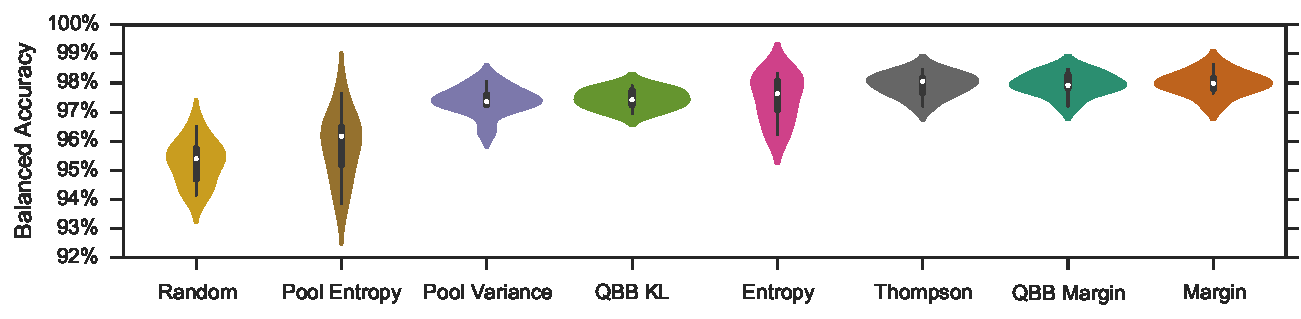
\includegraphics[width=\textwidth]{figures/5_active/vstatlas_bl_ind_violin}
		\caption{Balanced unlabelled pool and logistic regression}
		\label{fig:vstatlas_bl_ind_violin}
	\end{subfigure}\\
	\begin{subfigure}{\textwidth}
		\centering
		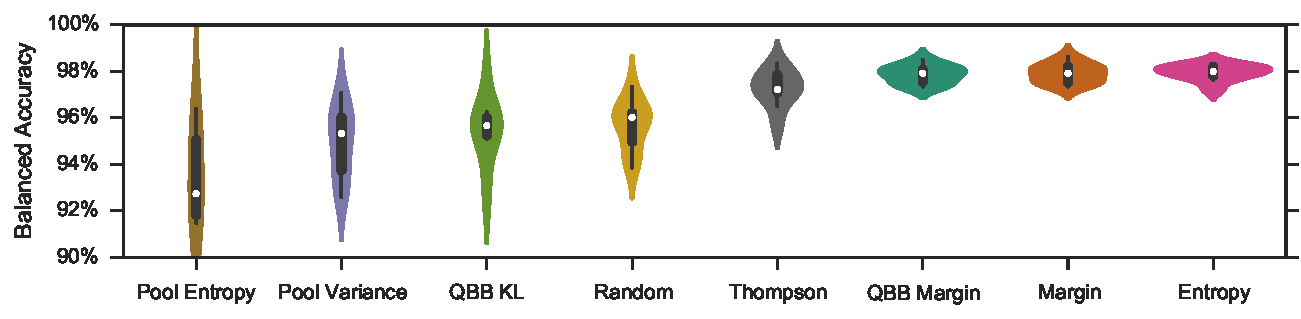
\includegraphics[width=\linewidth]{figures/5_active/vstatlas_br_ind_violin}
		\caption{Balanced unlabelled pool and RBF SVM}
		\label{fig:vstatlas_br_ind_violin}
	\end{subfigure}\\
	\begin{subfigure}{\textwidth}
		\centering
		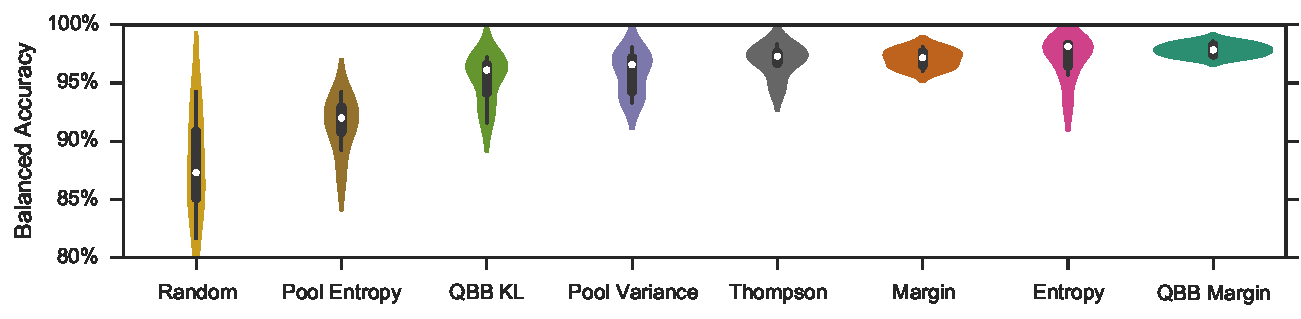
\includegraphics[width=\textwidth]{figures/5_active/vstatlas_ul_ind_violin}
		\caption{Unbalanced unlabelled pool and logistic regression}
		\label{fig:vstatlas_ul_ind_violin}
	\end{subfigure}\\
	\begin{subfigure}{\textwidth}
		\centering
		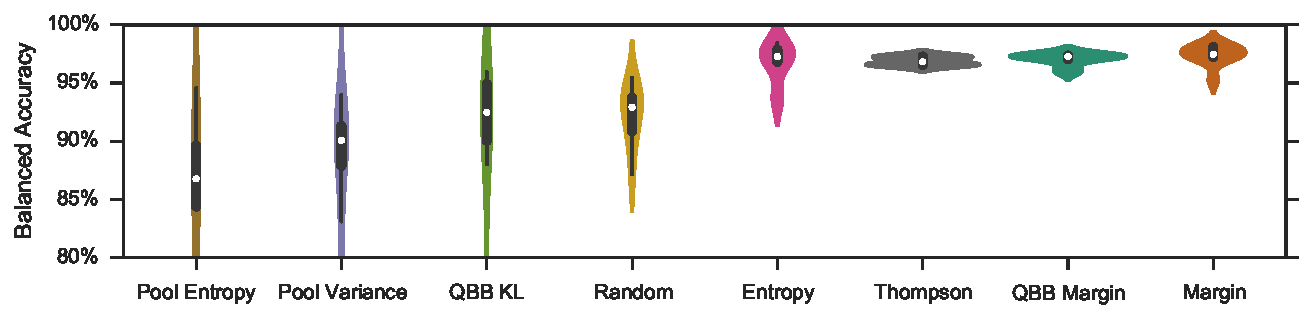
\includegraphics[width=\linewidth]{figures/5_active/vstatlas_ur_ind_violin}
		\caption{Unbalanced unlabelled pool and RBF SVM}
		\label{fig:vstatlas_ur_ind_violin}
	\end{subfigure}
	\caption[Violin plots of balanced accuracy (VST ATLAS)]{
		Posterior distributions of the balanced accuracy when the VST ATLAS training set size reaches 300: Overall, all heuristics outperform random sampling when we use logistic regression. With RBF SVM, the two pool heuristics and QBB KL do not seem to do as well.
		In particular, as we can see in Figure \ref{fig:vstatlas_ur_ind_violin}, when the classes are unbalanced, these three heuristics become very unreliable.}
	\label{fig:vstatlas_bl_ind}
\end{figure}


\begin{figure}[p]
	\centering
	\begin{subfigure}{.5\textwidth}
		\centering
		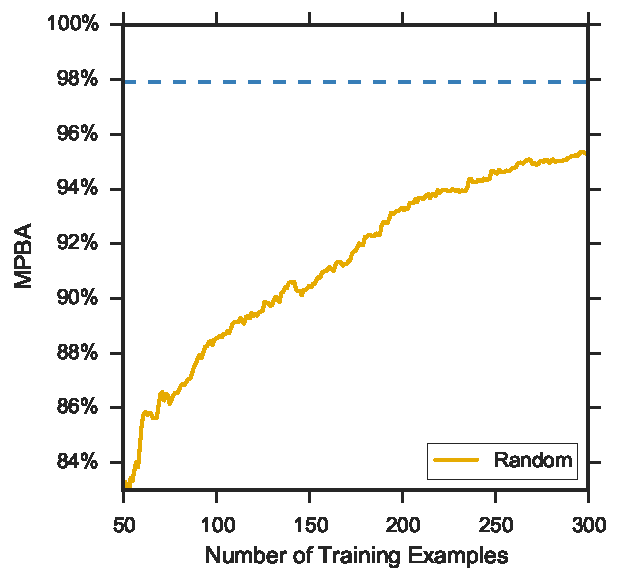
\includegraphics[width=\textwidth]{figures/5_active/vstatlas_bl_ind_lower}
		\caption{Balanced pool and logistic regression}
		\label{fig:vstatlas_bl_ind_lower}
	\end{subfigure}%
	\begin{subfigure}{.5\textwidth}
		\centering
		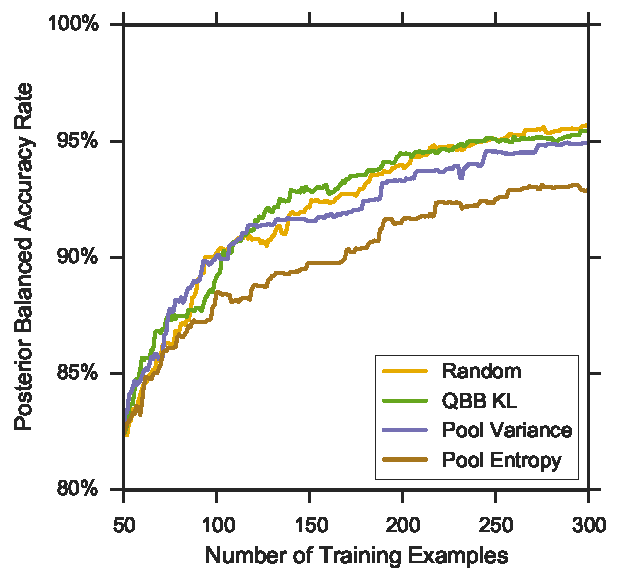
\includegraphics[width=\linewidth]{figures/5_active/vstatlas_br_ind_lower}
		\caption{Balanced pool and RBF SVM}
		\label{fig:vstatlas_br_ind_lower}
	\end{subfigure}
	\begin{subfigure}{.5\textwidth}
		\centering
		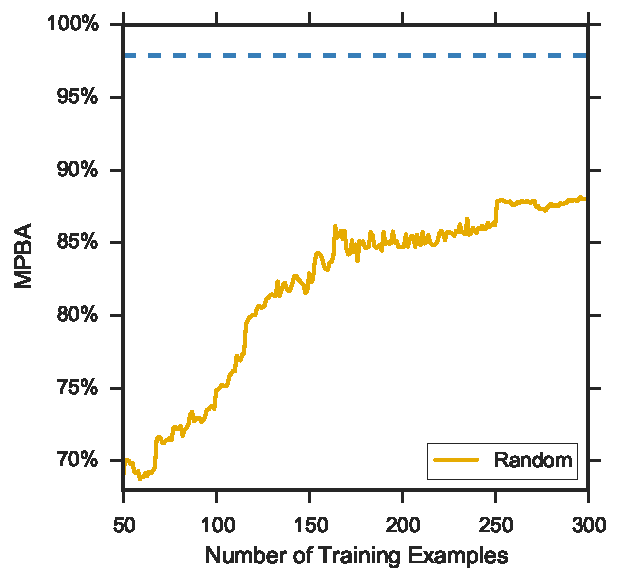
\includegraphics[width=\textwidth]{figures/5_active/vstatlas_ul_ind_lower}
		\caption{Unbalanced pool and logistic regression}
		\label{fig:vstatlas_ul_ind_lower}
	\end{subfigure}%
	\begin{subfigure}{.5\textwidth}
		\centering
		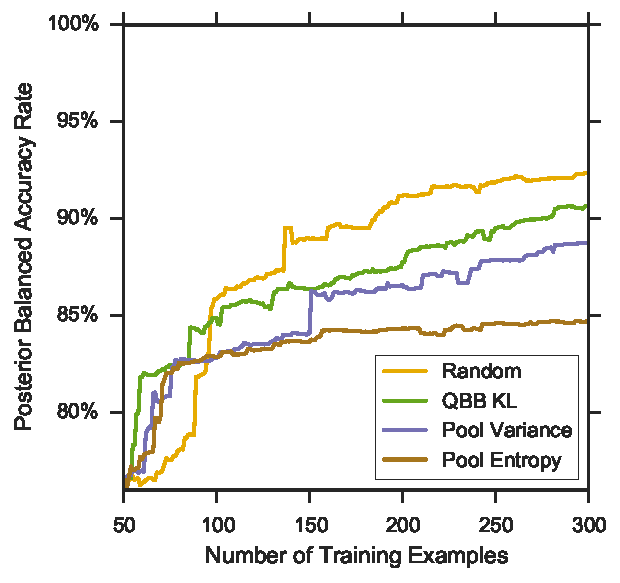
\includegraphics[width=\linewidth]{figures/5_active/vstatlas_ur_ind_lower}
		\caption{Unbalanced pool and RBF SVM}
		\label{fig:vstatlas_ur_ind_lower}
	\end{subfigure}
	\caption[Learning curves of heuristics worse than random (VST ATLAS)]{
		Learning curves (average of 10 trials) of heuristics that perform worse than random sampling in the VST ATLAS dataset: The plots for logistic regression are quite uninteresting
		since all heuristics beat random sampling. In Figure \ref{fig:vstatlas_ur_ind_lower},
		the learning curve for the pool entropy heuristic appears to flatten out after 100 samples.
		}
	\label{fig:vstatlas_ind_lower}
\end{figure}


\begin{figure}[p]
	\centering
	\begin{subfigure}{.5\textwidth}
		\centering
		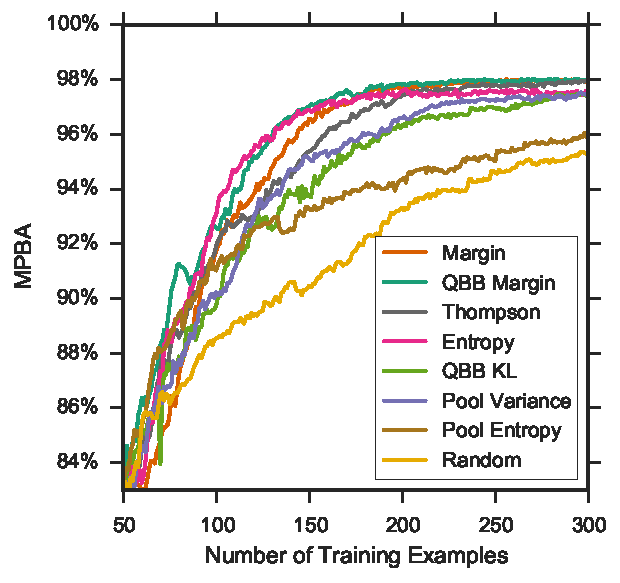
\includegraphics[width=\textwidth]{figures/5_active/vstatlas_bl_ind_upper}
		\caption{Balanced pool and logistic regression}
		\label{fig:vstatlas_bl_ind_upper}
	\end{subfigure}%
	\begin{subfigure}{.5\textwidth}
		\centering
		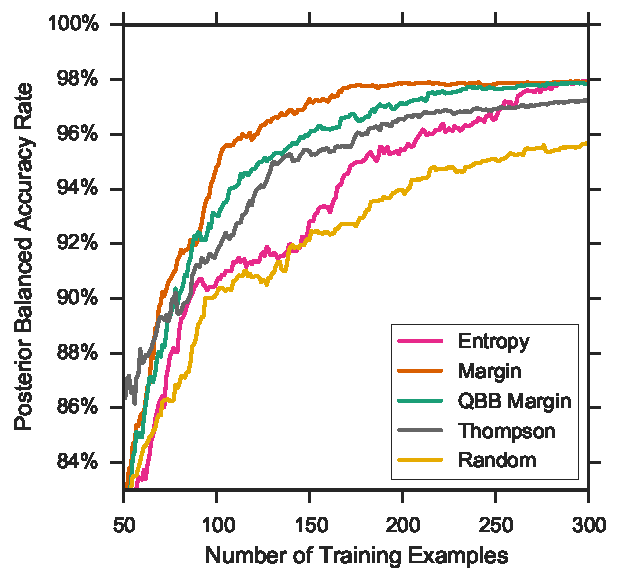
\includegraphics[width=\linewidth]{figures/5_active/vstatlas_br_ind_upper}
		\caption{Balanced pool and RBF SVM}
		\label{fig:vstatlas_br_ind_upper}
	\end{subfigure}
	\begin{subfigure}{.5\textwidth}
		\centering
		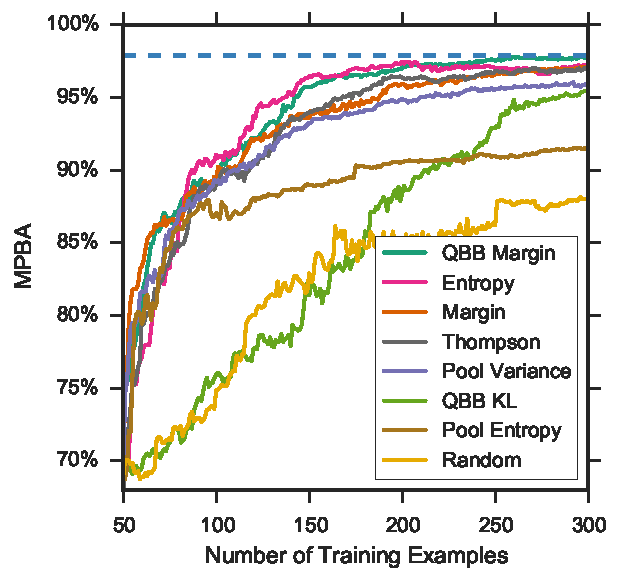
\includegraphics[width=\textwidth]{figures/5_active/vstatlas_ul_ind_upper}
		\caption{Unbalanced pool and logistic regression}
		\label{fig:vstatlas_ul_ind_upper}
	\end{subfigure}%
	\begin{subfigure}{.5\textwidth}
		\centering
		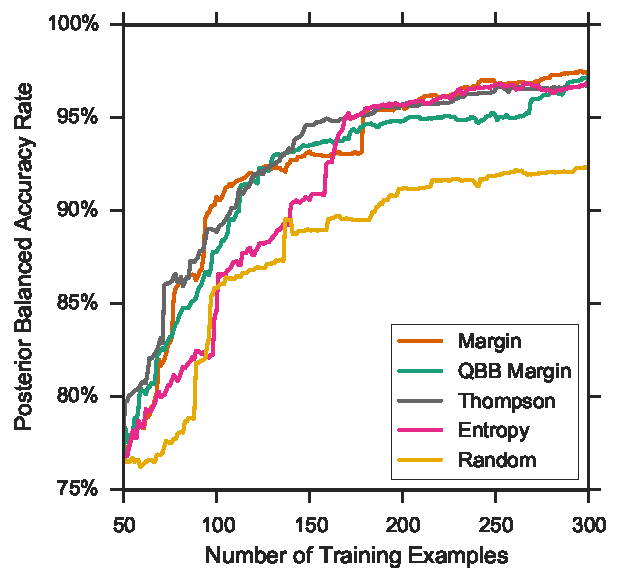
\includegraphics[width=\linewidth]{figures/5_active/vstatlas_ur_ind_upper}
		\caption{Unbalanced pool and RBF SVM}
		\label{fig:vstatlas_ur_ind_upper}
	\end{subfigure}
	\caption[Learning curves of heuristics better than random (VST ATLAS)]{
		Learning curves (average of 10 trials) of heuristics that outperform random sampling in the VST ATLAS dataset: It is great to see that with logistic regression, we have basically reached
        the maximum accuracy (indicated by the dashed line) after only 200 samples.
	}
	\label{fig:vstatlas_ind_upper}
\end{figure}


\begin{figure}[p]
    \centering
    \begin{subfigure}{.5\textwidth}
        \centering
        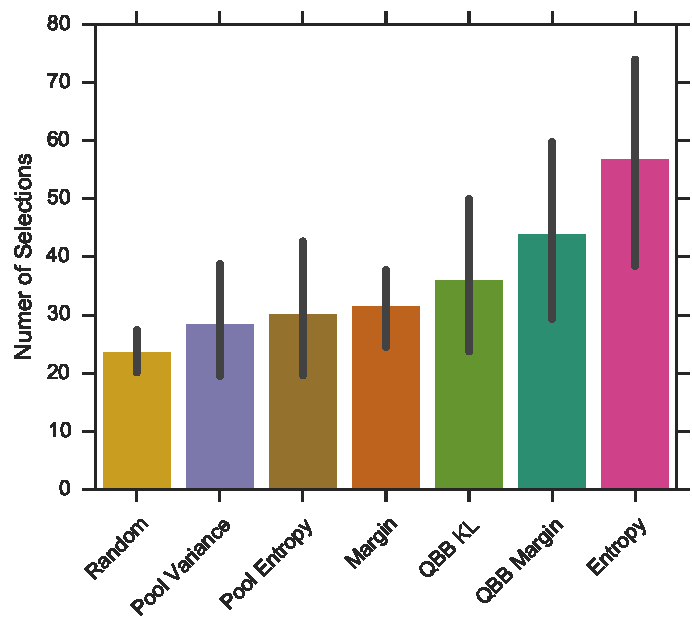
\includegraphics[width=\textwidth]{figures/5_thompson/vstatlas_bl_no_selections}
        \caption{Balanced pool and logistic regression}
        \label{fig:vstatlas_bl_no_selections}
    \end{subfigure}%
    \begin{subfigure}{.5\textwidth}
        \centering
        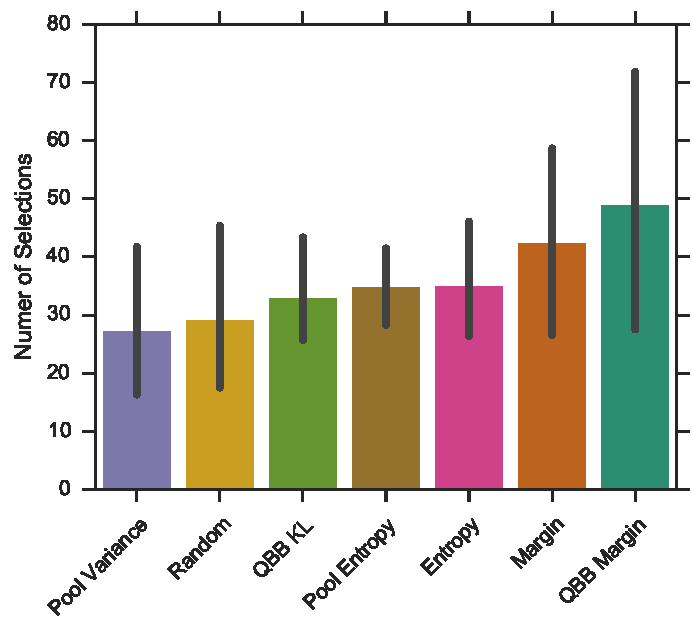
\includegraphics[width=\linewidth]{figures/5_thompson/vstatlas_br_no_selections}
        \caption{Balanced pool and RBF SVM}
        \label{fig:vstatlas_br_no_selections}
    \end{subfigure}
    \begin{subfigure}{.5\textwidth}
        \centering
        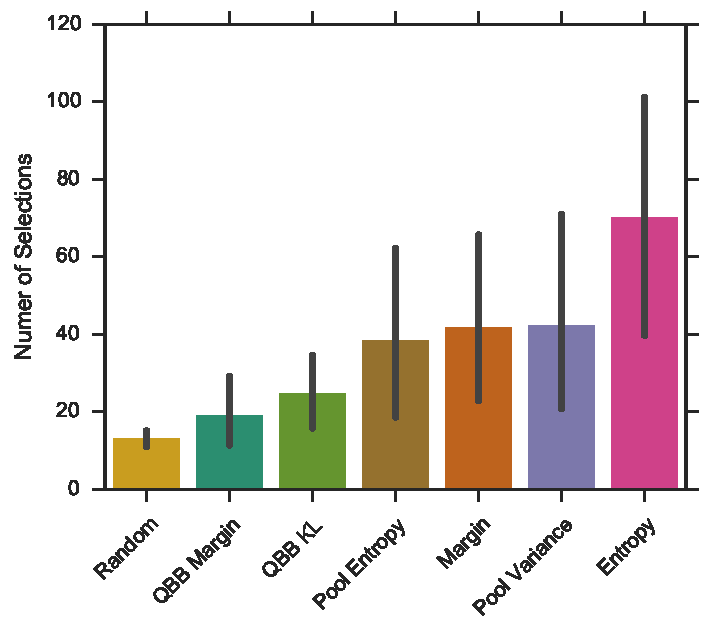
\includegraphics[width=\textwidth]{figures/5_thompson/vstatlas_ul_no_selections}
        \caption{Unbalanced pool and logistic regression}
        \label{fig:vstatlas_ul_no_selections}
    \end{subfigure}%
    \begin{subfigure}{.5\textwidth}
        \centering
        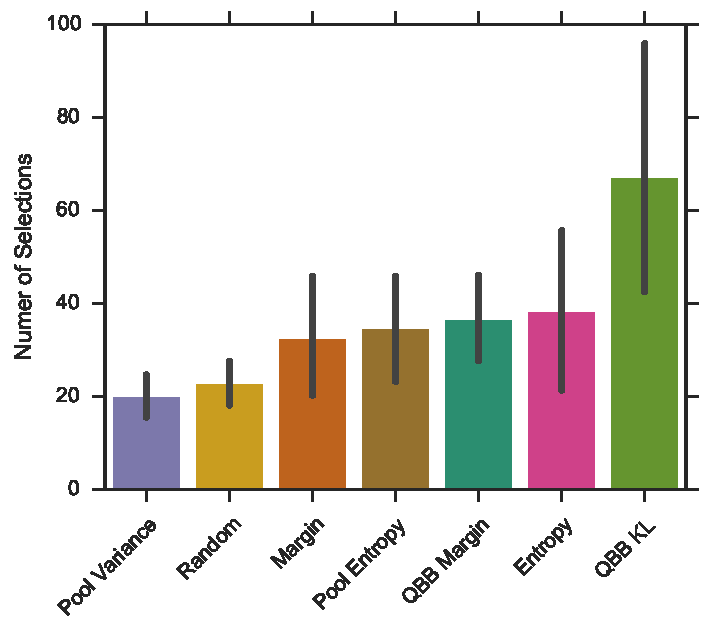
\includegraphics[width=\linewidth]{figures/5_thompson/vstatlas_ur_no_selections}
        \caption{Unbalanced pool and RBF SVM}
        \label{fig:vstatlas_ur_no_selections}
    \end{subfigure}
    \caption[Total number of heuristic selections (VST ATLAS)]{Total number of selections (average
        of 10 trials) of the six heuristics in Thompson sampling with the VST ATLAS dataset: Like the
        SDSS, it seems that most of the time, Thompson sampling manages to select the better
        heuristics more often than average, while maintaining a good exploration. There are also a few
        anomalies. For example with an unbalanced pool and RBF SVM, QBB KL is picked the most number of times. However when we study it individually, it performs worse than random sampling. And yet, Thompson sampling still finishes third, as shown in Figure \ref{fig:vstatlas_ur_ind_upper}. Thus a small amount of false belief seems to not be a problem.}
    
    \label{fig:vstatlas_no_selections}
\end{figure}


\begin{figure}[p]
	\centering
	\begin{subfigure}{.5\textwidth}
		\centering
		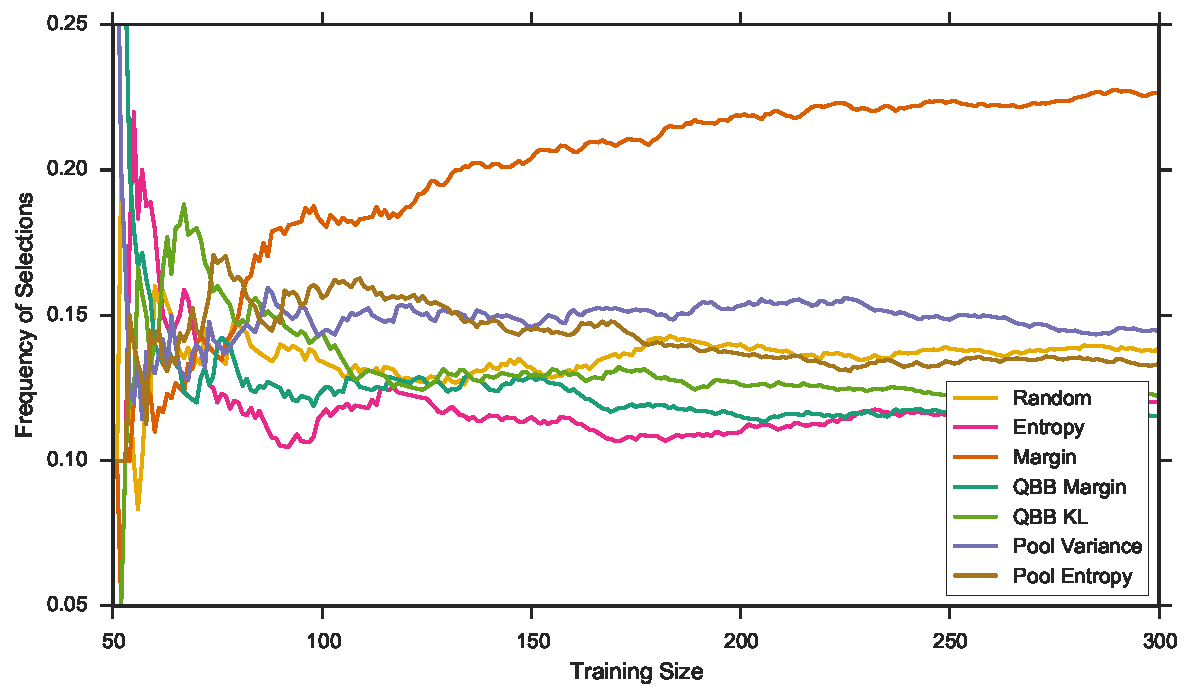
\includegraphics[width=\textwidth]{figures/5_thompson/vstatlas_bl_frequencies}
		\caption{Balanced pool and logistic regression}
		\label{fig:vstatlas_bl_frequencies}
	\end{subfigure}%
	\begin{subfigure}{.5\textwidth}
		\centering
		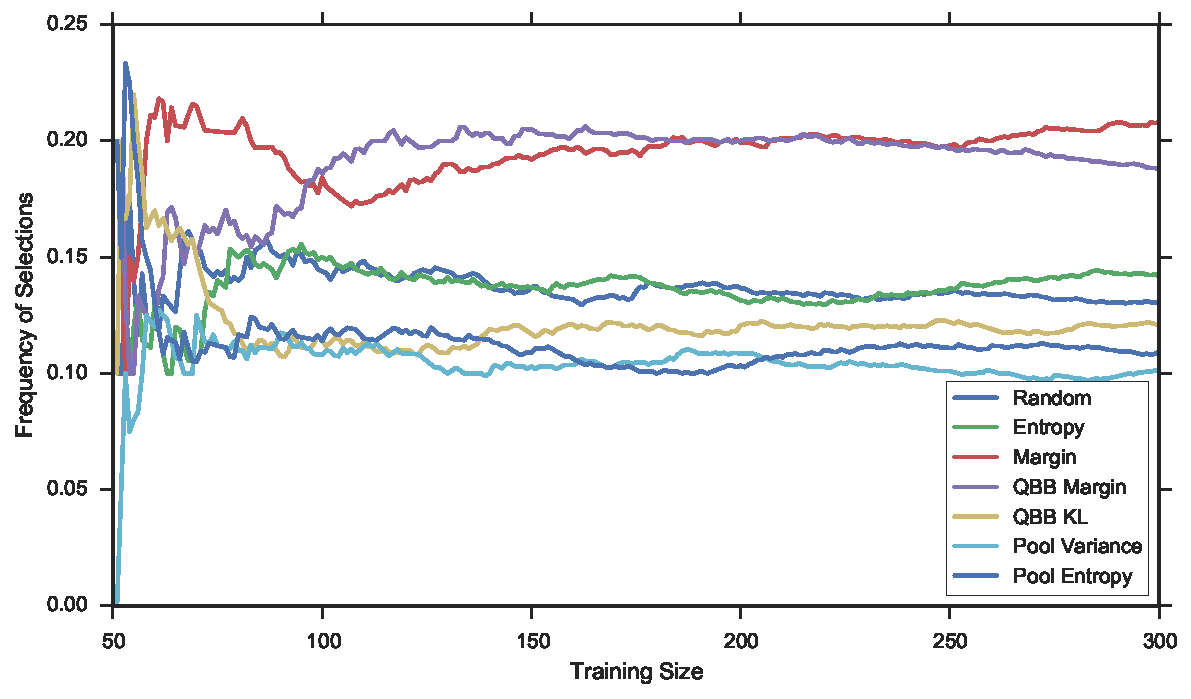
\includegraphics[width=\linewidth]{figures/5_thompson/vstatlas_br_frequencies}
		\caption{Balanced pool and RBF SVM}
		\label{fig:vstatlas_br_frequencies}
	\end{subfigure}
	\begin{subfigure}{.5\textwidth}
		\centering
		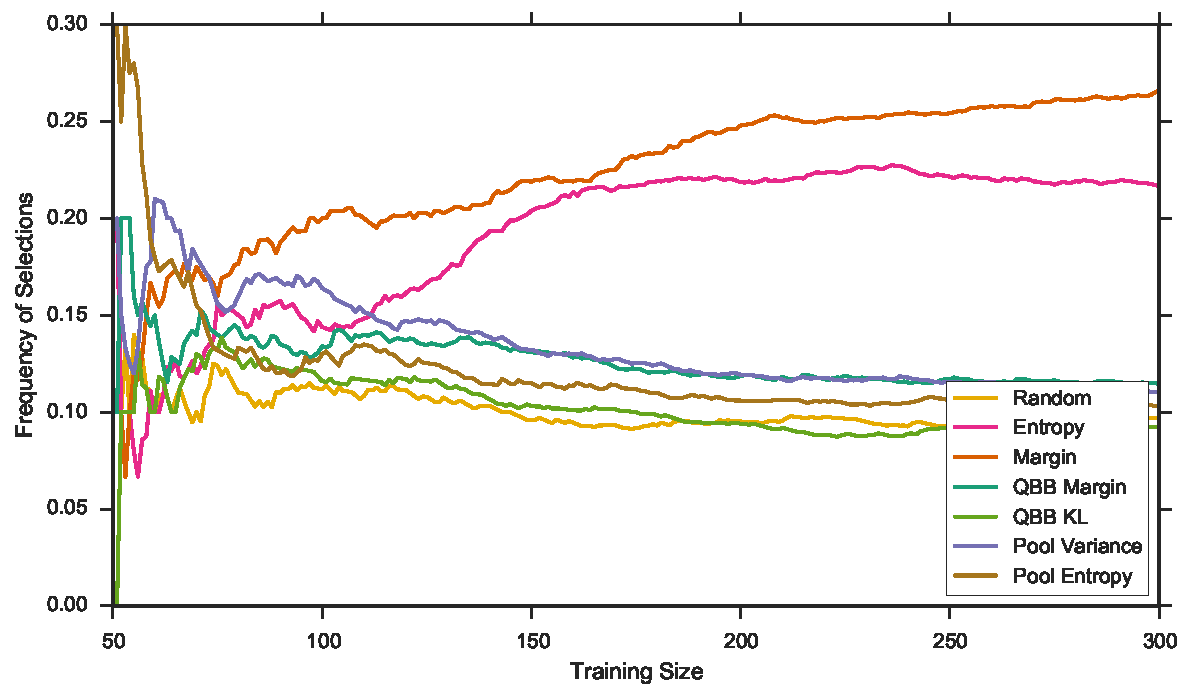
\includegraphics[width=\textwidth]{figures/5_thompson/vstatlas_ul_frequencies}
		\caption{Unbalanced pool and logistic regression}
		\label{fig:vstatlas_ul_frequencies}
	\end{subfigure}%
	\begin{subfigure}{.5\textwidth}
		\centering
		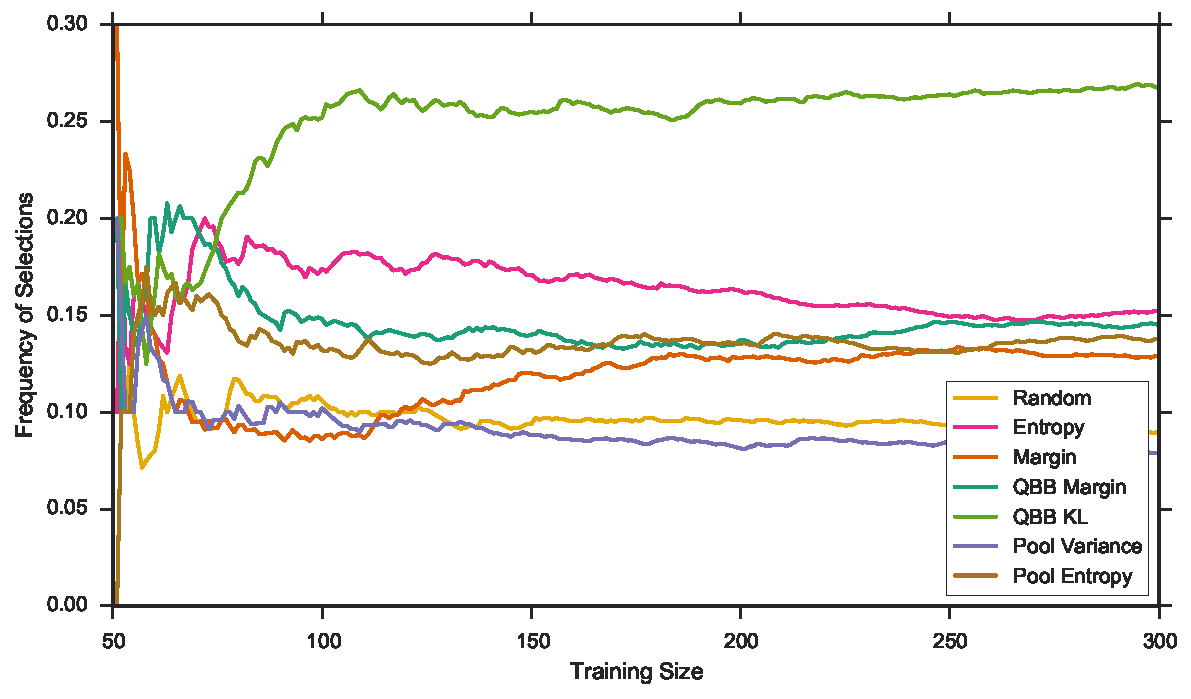
\includegraphics[width=\linewidth]{figures/5_thompson/vstatlas_ur_frequencies}
		\caption{Unbalanced pool and RBF SVM}
		\label{fig:vstatlas_ur_frequencies}
	\end{subfigure}
	\caption[Heuristic selection frequency (VST ATLAS)]{
		Heuristic selection frequency (average of 10 trials) in Thompson sampling with the VST ATLAS dataset.}
	\label{fig:vstatlas_frequencies}
\end{figure}


\begin{figure}[p]
	\centering
	\begin{subfigure}{.5\textwidth}
		\centering
		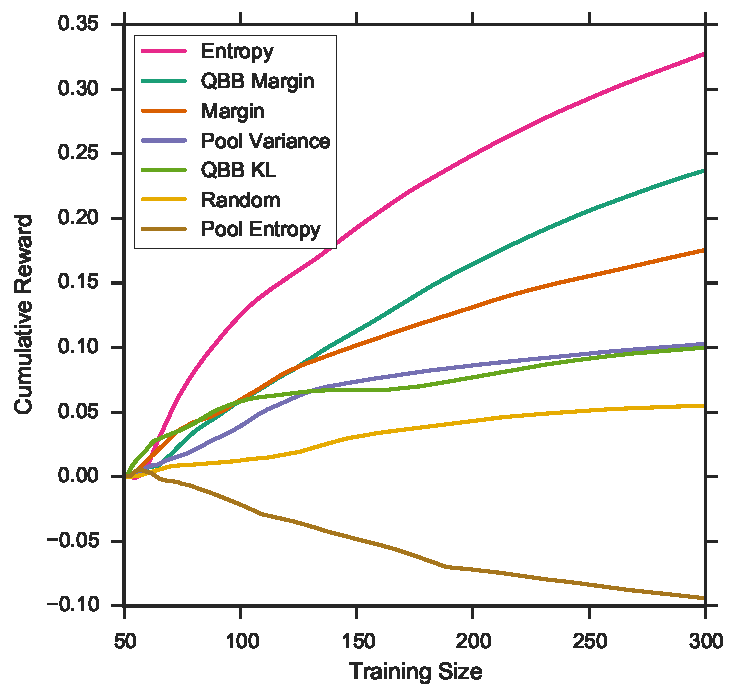
\includegraphics[width=\textwidth]{figures/5_thompson/vstatlas_bl_sum_rewards}
		\caption{Balanced pool and logistic regression}
		\label{fig:vstatlas_bl_sum_rewards}
	\end{subfigure}%
	\begin{subfigure}{.5\textwidth}
		\centering
		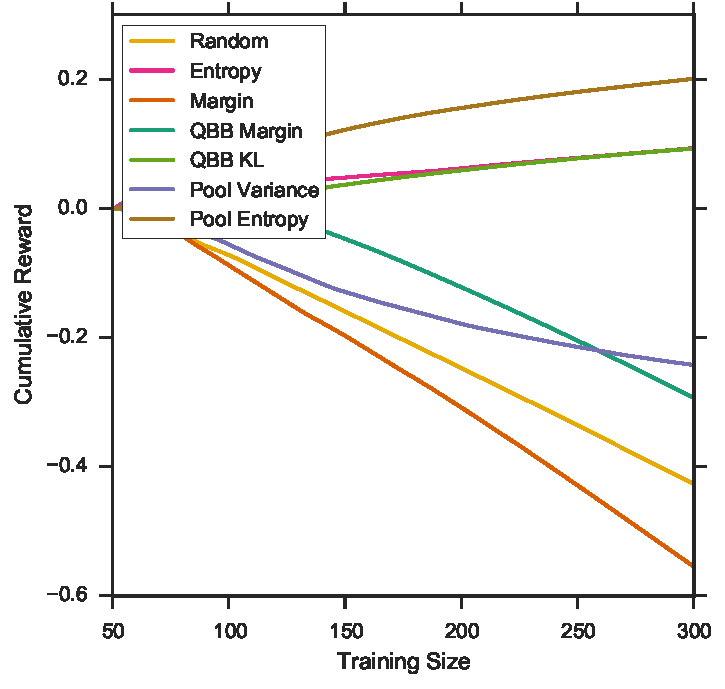
\includegraphics[width=\linewidth]{figures/5_thompson/vstatlas_br_sum_rewards}
		\caption{Balanced pool and RBF SVM}
		\label{fig:vstatlas_br_sum_rewards}
	\end{subfigure}
	\begin{subfigure}{.5\textwidth}
		\centering
		\includegraphics[width=\textwidth]{figures/5_thompson/vstatlas_ul_sum_rewards}
		\caption{Unbalanced pool and logistic regression}
		\label{fig:vstatlas_ul_sum_rewards}
	\end{subfigure}%
	\begin{subfigure}{.5\textwidth}
		\centering
		\includegraphics[width=\linewidth]{figures/5_thompson/vstatlas_ur_sum_rewards}
		\caption{Unbalanced pool and RBF SVM}
		\label{fig:vstatlas_ur_sum_rewards}
	\end{subfigure}
	\caption[Cumulative reward of heuristics (VST ATLAS)]{
		Cumulative reward (average of 10 trials) in Thompson sampling with the VST ATLAS dataset.}
	\label{fig:vstatlas_sum_rewards}
\end{figure}


\begin{figure}[p]
	\centering
	\begin{subfigure}{.5\textwidth}
		\centering
		\includegraphics[width=\textwidth]{figures/5_thompson/vstatlas_bl_avg_rewards}
		\caption{Balanced pool and logistic regression}
		\label{fig:vstatlas_bl_avg_rewards}
	\end{subfigure}%
	\begin{subfigure}{.5\textwidth}
		\centering
		\includegraphics[width=\linewidth]{figures/5_thompson/vstatlas_br_avg_rewards}
		\caption{Balanced pool and RBF SVM}
		\label{fig:vstatlas_br_avg_rewards}
	\end{subfigure}
	\begin{subfigure}{.5\textwidth}
		\centering
		\includegraphics[width=\textwidth]{figures/5_thompson/vstatlas_ul_avg_rewards}
		\caption{Unbalanced pool and logistic regression}
		\label{fig:vstatlas_ul_avg_rewards}
	\end{subfigure}%
	\begin{subfigure}{.5\textwidth}
		\centering
		\includegraphics[width=\linewidth]{figures/5_thompson/vstatlas_ur_avg_rewards}
		\caption{Unbalanced pool and RBF SVM}
		\label{fig:vstatlas_ur_avg_rewards}
	\end{subfigure}
	\caption[Mean reward (average of 10 trials) of heuristics (VST ATLAS)]{
		Mean reward in Thompson sampling with the VST ATLAS dataset.}
	\label{fig:vstatlas_avg_rewards}
\end{figure}
%%% Local Variables: 
%%% mode: latex
%%% TeX-master: "thesis"
%%% End: 
